% ============================================================
%  SCIENCE FLUX CLASSES  |  RBSE Class 12  |  PHYSICS BLACK BOOK
%  Front cover  -  A4, full bleed, CMYK-safe black & gold
%  Build:  xelatex cover.tex
% ============================================================
\documentclass[a4paper]{article}
\usepackage[a4paper,margin=0pt]{geometry}
\usepackage{fontspec}
\usepackage{xcolor}
\usepackage{tikz}
\usepackage{graphicx}
\usetikzlibrary{calc,shapes.misc,decorations.markings,shadings,fadings,positioning,arrows.meta}
\pagestyle{empty}
\setlength{\parindent}{0pt}

% ---------- fonts ----------
\newfontfamily\hero[Path=/usr/share/fonts/opentype/inter/,Extension=.otf]{InterDisplay-Black}
\newfontfamily\heroBold[Path=/usr/share/fonts/opentype/inter/,Extension=.otf]{InterDisplay-ExtraBold}
\newfontfamily\ui[Path=/usr/share/fonts/opentype/inter/,Extension=.otf,
  BoldFont=Inter-Bold,ItalicFont=Inter-Italic,BoldItalicFont=Inter-BoldItalic]{Inter-Medium}
\newfontfamily\uiSemi[Path=/usr/share/fonts/opentype/inter/,Extension=.otf]{Inter-SemiBold}
\newfontfamily\uiBold[Path=/usr/share/fonts/opentype/inter/,Extension=.otf]{Inter-Bold}
\newfontfamily\uiBlack[Path=/usr/share/fonts/opentype/inter/,Extension=.otf]{Inter-Black}
\newfontfamily\hook{FiraSans-HeavyItalic.otf}
\newfontfamily\hookLight{FiraSans-MediumItalic.otf}

% ---------- palette ----------
\definecolor{ink}{HTML}{070707}
\definecolor{ink2}{HTML}{111111}
\definecolor{ink3}{HTML}{1C1C1C}
\definecolor{gold}{HTML}{D4AF37}
\definecolor{goldL}{HTML}{F3D97C}
\definecolor{goldD}{HTML}{9C7A1E}
\definecolor{cream}{HTML}{F5EFDF}
\definecolor{mist}{HTML}{BFBFBF}
\definecolor{wa}{HTML}{25D366}
\definecolor{yt}{HTML}{FF0000}
\definecolor{sky}{HTML}{4FC3F7}
\definecolor{ember}{HTML}{FF7A1A}

% ---------- small helpers ----------
\newcommand{\pill}[5]{% x y fill textcolor text
  \node[fill=#3,rounded corners=2.2mm,inner xsep=3.2mm,inner ysep=1.5mm,anchor=west,
        text=#4,font=\uiBold\fontsize{10.5}{12}\selectfont] at (#1mm,#2mm) {#5};}

% chapter icon ring:  \iconring{x}{y}{label}{drawing code}
\newcommand{\iconring}[4]{%
  \begin{scope}[shift={(#1mm,#2mm)}]
    \shade[inner color=gold!35!ink,outer color=ink,opacity=.9] (0,0) circle (13.5mm);
    \fill[ink2] (0,0) circle (11.2mm);
    \draw[gold,line width=1.1pt] (0,0) circle (11.2mm);
    \draw[goldD,line width=.35pt] (0,0) circle (12.3mm);
    \begin{scope}[scale=.16,line cap=round,line join=round]
      #4
    \end{scope}
    \node[text=cream,font=\uiSemi\fontsize{9.5}{10}\selectfont,anchor=north] at (0,-12.8mm) {#3};
  \end{scope}}

% stat tile:  \stat{x}{y}{big}{line1}{line2}
\newcommand{\stat}[5]{%
  \begin{scope}[shift={(#1mm,#2mm)}]
    \fill[ink2,rounded corners=3mm] (0,0) rectangle (56mm,27mm);
    \draw[goldD!70!ink,line width=.6pt,rounded corners=3mm] (0,0) rectangle (56mm,27mm);
    \fill[gold] (0,5mm) rectangle (1.4mm,22mm);
    \node[anchor=base west,text=goldL,font=\hero\fontsize{26}{26}\selectfont,inner sep=0] at (5.5mm,14.5mm) {#3};
    \node[anchor=base west,text=white,font=\uiBold\fontsize{11}{12}\selectfont,inner sep=0] at (5.5mm,8.6mm) {#4};
    \node[anchor=base west,text=mist,font=\ui\fontsize{8.6}{9}\selectfont,inner sep=0] at (5.5mm,4.2mm) {#5};
  \end{scope}}

\begin{document}
\begin{tikzpicture}[remember picture,overlay,shift={(current page.south west)},x=1mm,y=1mm]

% =================== BACKGROUND ===================
\fill[ink] (0,0) rectangle (210,297);
% soft gold glow behind the atom
\shade[inner color=gold!22!ink,outer color=ink] (168,196) circle (95);
% faint dot grid texture
\foreach \i in {6,12,...,204}{\foreach \j in {6,12,...,294}{\fill[white,opacity=.045] (\i,\j) circle (.22);}}
% diagonal foil sweep (very subtle)
\fill[gold,opacity=.035] (0,120) -- (210,205) -- (210,230) -- (0,145) -- cycle;

% =================== ATOM MOTIF (TikZ) ===================
\begin{scope}[shift={(166,198)}]
  % glow rings
  \foreach \a in {0,60,120}{
    \draw[gold,opacity=.10,line width=5pt,rotate=\a] (0,0) ellipse (52 and 17);
    \draw[gold,opacity=.55,line width=1.1pt,rotate=\a] (0,0) ellipse (52 and 17);
    \draw[goldL,opacity=.9,line width=.4pt,rotate=\a] (0,0) ellipse (52 and 17);
  }
  % electrons (parametric points on the ellipses)
  \foreach \a/\t/\c in {0/40/sky, 60/200/goldL, 120/300/sky, 0/215/ember, 120/95/goldL}{
    \begin{scope}[rotate=\a]
      \shade[inner color=\c,outer color=\c!10!ink,opacity=.75] ({52*cos(\t)},{17*sin(\t)}) circle (3.4);
      \fill[\c] ({52*cos(\t)},{17*sin(\t)}) circle (1.55);
      \fill[white] ({52*cos(\t)-.5},{17*sin(\t)+.5}) circle (.45);
    \end{scope}}
  % nucleus
  \shade[inner color=goldL,outer color=gold!15!ink,opacity=.9] (0,0) circle (9);
  \shade[ball color=gold] (0,0) circle (4.6);
  \fill[white,opacity=.55] (-1.3,1.5) circle (1.1);
\end{scope}

% =================== LEFT SPINE BAND ===================
\fill[gold] (0,0) rectangle (9.5,262);
\fill[goldD] (9.5,0) rectangle (10.3,262);
\node[rotate=90,anchor=center,text=ink,font=\uiBlack\fontsize{11.5}{12}\selectfont,inner sep=0]
  at (4.9,131) {RBSE \ \textbullet\ \ CLASS 12 \ \textbullet\ \ SESSION 2026–27 \ \textbullet\ \ BOARD EXAM 2027 \ \textbullet\ \ ENGLISH MEDIUM};

% =================== HEADER ===================
\fill[ink2] (0,262) rectangle (210,297);
\fill[gold] (0,261.2) rectangle (210,262.6);
\fill[goldD] (0,260) rectangle (210,260.6);
\node[anchor=center] at (24,279.5) {
\includegraphics[width=27mm]{assets/sfc_logo.png}};
\draw[gold,line width=.9pt] (24,279.5) circle (14.2);
\node[anchor=west,text=white,font=\hero\fontsize{25}{26}\selectfont,inner sep=0] at (42,284.5) {SCIENCE FLUX CLASSES};
\draw[gold,line width=1.1pt] (42,277.3) -- (150,277.3);
\node[anchor=west,text=goldL,font=\hookLight\fontsize{12.5}{13}\selectfont,inner sep=0] at (42.3,272.4) {Pure Quality \ \textbullet\ \ Pure Satisfaction};
\node[fill=gold,rounded corners=2mm,inner xsep=3mm,inner ysep=1.6mm,anchor=east,text=ink,font=\uiBlack\fontsize{10}{11}\selectfont] at (203,285) {ENGLISH MEDIUM};
\node[draw=gold,rounded corners=2mm,inner xsep=3mm,inner ysep=1.5mm,anchor=east,text=goldL,font=\uiBold\fontsize{9.5}{11}\selectfont,line width=.6pt] at (203,272.5) {QUESTION BANK};

% =================== HERO ===================
\pill{18}{246}{gold}{ink}{RBSE \ \textbullet\ \ CLASS 12 \ \textbullet\ \ NCERT LINE-TO-LINE}
\node[fill=ink,draw=gold,line width=.6pt,rounded corners=2.2mm,inner xsep=3.2mm,inner ysep=1.5mm,anchor=west,text=goldL,font=\uiBold\fontsize{10.5}{12}\selectfont] at (102mm,246mm) {BOARD EXAM 2027};
% PHYSICS  (resized to a fixed width so it can never overflow)
\node[anchor=south west,inner sep=0,text=white] at (17,199.5) {\hero\resizebox{152mm}{!}{PHYSICS}};
% BLACK BOOK
\node[anchor=south west,inner sep=0,text=gold] at (17.5,176) {\hero\resizebox{112mm}{!}{BLACK BOOK}};
\draw[gold,line width=1.6pt] (18,172.5) -- (78,172.5);
\draw[goldD,line width=.5pt] (78,172.5) -- (150,172.5);

% signature line (sticker)
\node[fill=gold,rounded corners=1.2mm,inner xsep=3.6mm,inner ysep=1.9mm,anchor=west,rotate=-1.5,
      text=ink,font=\hook\fontsize{19}{20}\selectfont] at (18,163) {“Iske Bahar Kuch Nahi!”};
% the buy line
\node[anchor=west,text=white,font=\hook\fontsize{15}{16}\selectfont,inner sep=0] at (18.5,150.5)
  {Jo Paper Mein Aayega, \textcolor{goldL}{Yahin Se Aayega.}};

% =================== STAT TILES ===================
\stat{18}{111}{16}{Years of PYQ}{RBSE 2011–2026, year-tagged}
\stat{78}{111}{100\%}{NCERT Line-to-Line}{Every line, table \& figure}
\stat{138}{111}{1}{Book. Full Marks.}{Every answer, right inside}

% =================== CHAPTER ICONS ===================
\iconring{30}{78}{Electricity}{%
  \draw[sky,line width=1.9pt] (-40,-22) -- (-40,22) -- (-14,22)
     -- (-10,30) -- (-4,14) -- (2,30) -- (8,14) -- (14,30) -- (18,22) -- (40,22) -- (40,-22) -- (6,-22);
  \draw[sky,line width=1.9pt] (-6,-22) -- (-40,-22);
  \draw[sky,line width=3pt] (-6,-32) -- (-6,-12);
  \draw[sky,line width=1.6pt] (6,-27) -- (6,-17);}
\iconring{60}{78}{Magnetism}{%
  \foreach \r in {14,26,38}{\draw[sky,line width=1.7pt] (0,0) circle (\r);}
  \foreach \r in {14,26,38}{\fill[sky] (\r,0) ++(-2.8,-4) -- (0,4) -- (2.8,-4) -- cycle;}
  \fill[yt] (0,0) circle (5);}
\iconring{90}{78}{AC Current}{%
  \draw[mist,line width=1.2pt,-{Stealth}] (-42,0) -- (44,0);
  \draw[mist,line width=1.2pt,-{Stealth}] (-36,-30) -- (-36,34);
  \draw[sky,line width=2pt,domain=-36:40,samples=60,smooth] plot (\x,{24*sin((\x+36)*9)});
  \draw[ember,line width=2pt,domain=-36:40,samples=60,smooth] plot (\x,{24*sin((\x+36)*9+90)});}
\iconring{120}{78}{Optics}{%
  \fill[sky,opacity=.35] (0,-36) .. controls (13,-12) and (13,12) .. (0,36) .. controls (-13,12) and (-13,-12) .. cycle;
  \draw[sky,line width=1.6pt] (0,-36) .. controls (13,-12) and (13,12) .. (0,36) .. controls (-13,12) and (-13,-12) .. cycle;
  \foreach \y in {-16,0,16}{\draw[yt,line width=1.6pt,-{Stealth}] (-44,\y) -- (-3,\y);}
  \foreach \y in {-16,0,16}{\draw[yt,line width=1.6pt] (3,\y) -- (40,0);}
  \fill[white] (40,0) circle (2.4);}
\iconring{150}{78}{Atoms \& Nuclei}{%
  \draw[sky,line width=1.5pt] (0,0) circle (18);
  \draw[sky,line width=1.5pt] (0,0) circle (32);
  \draw[sky,line width=1.5pt] (0,0) circle (44);
  \fill[yt] (0,0) circle (5.5);
  \fill[sky] (18,0) circle (3.2); \fill[sky] (-22,23) circle (3.2); \fill[sky] (31,-31) circle (3.2);
  \draw[ember,line width=1.8pt] (14,-8) -- (18,-14) -- (12,-17) -- (18,-24) -- (12,-27) -- (18,-33);}
\iconring{180}{78}{Semiconductors}{%
  \fill[yt!70!ink] (-26,4) rectangle (0,24); \fill[sky!60!ink] (0,4) rectangle (26,24);
  \draw[white,line width=1.2pt] (-26,4) rectangle (26,24);
  \node[text=white,font=\uiBold\fontsize{2.2}{2}\selectfont,scale=4] at (-13,14) {p};
  \node[text=white,font=\uiBold\fontsize{2.2}{2}\selectfont,scale=4] at (13,14) {n};
  \draw[white,line width=1.6pt] (-40,14) -- (-26,14); \draw[white,line width=1.6pt] (26,14) -- (40,14);
  \draw[white,line width=1.8pt] (-38,-22) -- (-8,-22) (10,-22) -- (40,-22);
  \fill[white] (-8,-10) -- (-8,-34) -- (10,-22) -- cycle;
  \draw[white,line width=2pt] (10,-10) -- (10,-34);}

% =================== FOOTER ===================
\shade[top color=ink,bottom color=ink3] (0,0) rectangle (210,48);
\fill[gold] (0,47.2) rectangle (210,48.4);
\fill[goldD] (0,46.4) rectangle (210,46.9);
% author
\node[anchor=center] at (30,24) {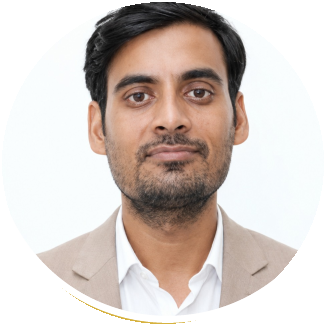
\includegraphics[width=33mm]{assets/nk_sir.png}};
\draw[gold,line width=1.6pt] (30,24) circle (17);
\node[anchor=west,text=goldL,font=\uiBold\fontsize{9.5}{10}\selectfont,inner sep=0] at (52,34) {BY};
\node[anchor=west,text=white,font=\hero\fontsize{21}{22}\selectfont,inner sep=0] at (52,26.5) {NanuRam Kumawat};
\node[anchor=west,text=gold,font=\hook\fontsize{13}{14}\selectfont,inner sep=0] at (52.3,17.5) {(NK Sir)};
\node[anchor=west,text=mist,font=\hookLight\fontsize{9.5}{10}\selectfont,inner sep=0] at (52.3,10.5) {Learn \ \textbullet\ \ Practice \ \textbullet\ \ Score};
\draw[goldD,line width=.5pt] (126,10) -- (126,38);
% WhatsApp
\begin{scope}[shift={(139,31)}]
  \fill[wa] (0,0) circle (4.6);
  \draw[white,line width=1.1pt] (0,0.2) circle (2.7);
  \fill[wa] (-2.9,-1.6) -- (-2.2,-3.7) -- (-.4,-2.4) -- cycle;
  \draw[white,line width=1.15pt,line cap=round] (-1.0,1.3) .. controls (-1.2,-.3) and (.4,-1.6) .. (1.5,-1.0);
\end{scope}
\node[anchor=west,text=mist,font=\ui\fontsize{8.5}{9}\selectfont,inner sep=0] at (147,34.2) {WhatsApp};
\node[anchor=west,text=white,font=\hero\fontsize{15}{16}\selectfont,inner sep=0] at (147,28) {8005777791};
% YouTube
\begin{scope}[shift={(139,15.5)}]
  \fill[yt,rounded corners=1.3mm] (-5,-3.3) rectangle (5,3.3);
  \fill[white] (-1.6,-2) -- (-1.6,2) -- (2.2,0) -- cycle;
\end{scope}
\node[anchor=west,text=mist,font=\ui\fontsize{8.5}{9}\selectfont,inner sep=0] at (147,19.2) {YouTube};
\node[anchor=west,text=white,font=\uiBlack\fontsize{12.5}{13}\selectfont,inner sep=0] at (147,13) {Science Flux Classes};

\end{tikzpicture}
\end{document}
